
\chapter{The Theory of Adjoint Systems}\label{chap2}

THIS\pageoriginale CHAPTER DEALS with the conductor $\underline{f}$ of
a reduced irreducible curve $C$ with respect to its normalisation
$\bar{C}$. The material is fairly classical, but we have developed it
from the point of view of duality. We will show that there is a very
simple relation between the conductor and the sheaf of differential
(or the dualising sheaf), namely
$$
\underline{f}=\varphi_*\omega_{\bar{C}}\otimes\omega_C^{-1},
$$
where $\varphi$ is the canonical morphism $\bar{C}\longrightarrow C$. 

From this fact and the computation of the dualising sheaf for the
blowing up of a point on a smooth surface, we get that, adjoint curves
are those, whose equation is in the `conductor'. The classical theorem
of Gorenstein (adjoints of degree $m-3$ cut out on $C$, the complete
canonical system of $\bar{C}$) is an easy consequence of the previous
considerations. So is the local formula $n=2\delta$. This point of
view introduces very naturally Kodaira's vanishing theorem. When one
tries to have a theorem similar to Gorenstein's, for a surface which
is not $\mathbb{P}^2$. We recommend to the interested reader,
Pathologies III \cite{key8} of D. Mumford, which contains a very nice
proof of the regularity of the adjoint system for a normal surface in
characteristic zero. In \S \ref{chap2:sec10} we give an example (char
$p>0$) of an ample divisor satisfying Kodaira's vanishing theorem, but
not the regularity of the adjoint system.

\section{Intersection Multiplicities}\label{chap2:sec1}
Let\pageoriginale $X$ be a projective, irreducible and non-singular
surface. Let $L_1$ and $L_2$ be two line bundles on $X$. Then we
define the {\it intersection multiplicity} of $L_1$ and $L_2$ denoted
by $(L_1.L_2)$ as  
$$
(L_1.L_2)=\chi(O_X)-\chi(L_1^{-1})-\chi(L_2^{-1})+\chi(L_1^{-1} 
\otimes L_2^{-1}).
$$

If $L_2=O_X(D)$ for some divisor $D$, then $(L_1,L_2)=\deg
(L_{1/D})$. Let $L_1=O_X(D_1)$ and $L_2=O_X(D_2)$ such that $D_1$ and
$D_2$ have no common components. Then,
$$
(L_1.L_2)=\sum\limits_{Q\in X}\quad\text{length}\quad(O_{D_1\cap
D_2,Q}). 
$$

The pairing $(- \cdotp -)$ is bilinear. 

\section{Blowing up a Closed Subscheme}\label{chap2:sec2}
 Let $X$ be
any scheme and $Y$ a closed subscheme of $X$. Let $J$ be the sheaf of
ideals of $Y$ in $O_X$.
\begin{def*}
The blowing up of $X$ with centre $Y$ is the scheme $Z=\Proj(O_X\oplus
J\oplus J^2\oplus\ldots)$. 
\end{def*}

We have a canonical morphism, $f:Z\longrightarrow X$ where $f$ is an
isomorphism of $Z-f^{-1}(Y)$ and $X-Y$. The blowing up has the
following universal property. The image $J.O_Z$ of $f^*J$ in $O_Z$ is
locally defined by one equation which is a non-zero divisor. If $W$ is
a scheme and $g:W\longrightarrow X$ a morphism such that the image of
$g^*J$ in $O_W$ is isomorphic to $O_W(-D)$ for some divisor $D$, then
$g$ factors through $Z$, \ie there exists a unique morphism
$h:W\longrightarrow Z$ such that the following diagram is commutative

\[
\xymatrix{
W \ar[r] \ar[d]_h & X\\
Z\ar[ur]_f 
}
\]

and the image of $h*(J.O_Z)$ in $O_W$ is equal to $O_W(-D)$. We recall
the definitions\pageoriginale of $g^*$ and $g_*$.

Let $g:X\longrightarrow Y$ be a morphism of schemes. Let $F$ be any
pre-sehaf on $X$. We define a pre-sehaf on $Y$ called $g_*F$ as
follows: $g_*F(U)=F(g^{-1}(U))$ for any open set in $Y$. One can check
that if $F$ is a sheaf, $g_*F$ is also a sheaf.

Let $G$ be a pre-sheaf on $Y$. Consider the functor
$F\longrightarrow\Hom (G,g_*F)$, from the category of pre-sheaves on
$X$ to the category of sets. If this functor is representable, we call
the pre-sheaf, $g^*G$.
$$
\Hom(F,g^*G)=\Hom(G,g_*F)\quad\text{for every pre-sheaf $F$ on $X$}.
$$

One can verify that in our case of $O_X$-modules this functor is
representable by an $O_X$-module ``associated to the following
pre-sheaf, for $U$ open in $Y,g^{-1}(U)=\Gamma(U,G)
\underset{\Gamma(U,O_y)}{\otimes}\Gamma(g^{-1}(U),O_X)$ 
\begin{def*}
The subscheme of $Z$ defined by the sheaf of ideal $(J.O_Z)$ is called
the {\it exceptional divisor} on $Z$ under the blowing up. It is equal
to $f^{-1}(Y)$. 
\end{def*}

Let $X$ be a non-singular, irreducible scheme of dimension 2. Let $P$
be a closed point on $X$. Let $\underline{M}$ denote the sheaf of
ideals defining $P$ in $O_X$. Let $X'$ be the blown up of $X$ at
$P$. So
$$
X'=\Proj(O_X\oplus\underline{M}^2\oplus\ldots)
$$
Let $E$ be the exceptional divisor. So 
\begin{align*}
E &= \Proj((O_X\oplus\underline{M}^2\oplus\ldots)\otimes\Spec O_X/
\underline{M})\\ 
&= \Proj (O_X/\underline{M}\oplus\underline{M}/\underline{M}^2 \oplus
\underline{M}^2/M_3\oplus\ldots)
\end{align*}
Since $X$ is non-singular surface and $\underline{M}$ is a maximal
ideal, we see that 
$$
E=\Proj(k[X,Y]=\mathbb{P}_k^1.
$$\pageoriginale

where $k$ is equal to the residue field of $P$. Hence
$$
O_X(E)_{/E}\quad\text{is equal to}\quad O_{\mathbb{P}^1}(-1)
$$
and the self intersection $(E.E)=-1$. 
\begin{REM*}
$X'$ is irreducible and non-singular.
\end{REM*}

\section{Canonical Divisor of the Blown up}\label{chap2:sec3} 
\begin{Prop*}
Let $X$ be a non-singular irreducible quasi-projective variety and $P$
any closed point of $X$. Let $X_1$ be the blown up of $X$ at $P$, and
$E$ the exceptional divisor. Let $f:X_1\longrightarrow X$ be the
blowing up map. If one denotes by $\omega_X(\resp\omega_{X_1})$ the
dualising sheaf $X(\resp\,\text{of}\, X_1)$ one has 
$$
\omega_{X_1}=f^*\omega_X\underset{O_{X_1}}{\otimes}O_{X_1}(E).
$$
\end{Prop*}

\begin{proof}
Let $L$ denote the line bundle
$\omega_{X_1}\underset{O_{X_1}}{\otimes}(f^*\omega_X)^{-1}$ Since $f$
is an isomorphism from $X_1-E$ to $X-P$, we see that $L_{/X_1-E}\simeq
O_{X_1-E}$. Since $X_1$ is non-singular $L=O_{X_1}(D)$ for some Weil
divisor $D$ on $X_1$. Let $D=D_1+\alpha E$ where $D_1$ does not have
$E$ as a component. Since $O_{X_1}(D)_{/X_1-E}$ is the trivial line
bundle we see that the divisor $D_1$ restricted to $X_1-E$ is
principal, \ie there exists a rational function $g$ on $X_1$ such that
$\Div(g)_{/X_1-E}=D_{1/X_1-E}$. So we see that $D_1-\Div(g)$ has only
$E$ as component and hence $D-\Div(g)$ also has only $E$ as its
component. So we get that $L=O_{X_1}(D)=O_{X_1}(D-\Div(g))=O_{X_1}(n
E)$ for some integer $n$. Thus 
$$
\omega_{X_1}\simeq f^*\omega_X\otimes O_{X_1}(n E).
$$

Now 
\begin{align*}
O_{\mathbb{P}^1}(-2) &= \omega_E=\omega_{X_1}\underset{O_{X_1}}
{\otimes} O_{X_1}(E)\underset{O_{X_1}}{\otimes}O_E\\
&= f^*\omega_X\underset{O_{X_1}}{\otimes}O_{X_1}((1+n)E)
\underset{O_{X_1}}{\otimes} O_E.
\end{align*}

Since\pageoriginale $E=f^*(P)$ and $\omega_X$ is trivial on $E$, we
see that $f^*\omega_X\underset{O_{X_1}}{\otimes}O_E=O_E$ So
$$
O_{\mathbb{P}^1}(-2)=O_{X_1}((1+n)E)\underset{O_{X_1}}{\otimes} O_E=
O_{\mathbb{P}^1}(-1(1+n)).
$$

Therefore $1+n=2$ or $n=1, \ie \omega_{X_1}=f^*\omega_X
\underset{O_{X_1}}{\otimes}\quad O_{X_1}(E)$.
\end{proof}

\section{Proper Transform}\label{chap2:sec4}
 Let $R$ be a regular local ring of dimension 2. Let $g$ be a non-zero
 element in the maximal ideal $M$ or $R$. We will calculate the
 Hilbert-Samuel function of the ring $A=R/_{(g)}$. 

Let us denote the maximal ideal of $A$ by
$\overline{M}$. $\overline{M}=M/_{gR}$. Let $g\in M^r-M^{r+1}$. Then
$$
\overline{M}^n=(M/gR)^n=M^n/gR\cap {M^n}.
$$

Since $g\in M^n$, for $n<r$,
$$
\overline{M}^n=M^n/{gR}.
$$

So, for $n<r$,
$$
\overline{M}^n/\overline{M}^{n+1} = M^n/gR \Big/ M^{n+1}/gR=
M^n/M^{n+1}.
$$

For $n>r$ we claim that $gR\cap M^n=g. M^{n-r}$. Clearly
$gM^{n-r}\subset gR\cap M^n$. Let $g.h\in M^n$, with $h\in
M^p-M^{p+1}$ Since the graded ring of $R$ is a domain, we see that
$p+r\geq n\,\ie p\geq n-r$. So $h\in M^{n-r}$ So for $n>r$, we have 
$$
\overline{M}^n/\overline{M}^{n+1} = M^n/gM^{n-r} \left/
M^{n+1}/gM^{n-r+1}  \right.
$$
We have an exact sequence of $k(=R/_M=A/_{\overline{M}})$ vector
spaces:
$$
0\longrightarrow\frac{gM^{n-r}}{gM^{n-r+1}} \longrightarrow
M^n/M^{n+1} \longrightarrow M^n/gM^{n-r} \left/M^{n+1}/gM^{n-r+1}
\longrightarrow 0. \right.
$$\pageoriginale

Since $\frac{gM^{n-r}}{gM^{n-r+1}}\simeq M^{n-r}/M^{n-r+1}$ we get,
\begin{align*}
\ell(\overline{M}^n/\overline{M}^{n+1}) &= \ell(M^n/M^{n+1})-
\ell(M^{n-r}/M^{n-r+1})\\
&= (n+1)-(n-r+1)=r.
\end{align*}
For $n<r, \ell(\overline{M}^n/_{\overline{M}^{n+1}})=\ell
(M^n/_{M^{n+1}})=n+1$. So, for $n<r$,
$$
\ell(A/_{\overline{M}^n})=\frac{n(n+1)}{2}
$$
and for $n>r$
$$
\ell(A/_{\overline{M}^n})=\frac{r(r+1)}{2}+(n-r).r=rn-\frac{r(r-1)}{2} 
$$
Thus we see that the Hilbert-Samuel polynomial is
$P(n)=rn-\frac{r(r-1)}{2}$ and, 
$$
\ell(A/_{\overline{M}^n})=P(n)\quad\text{for every}\quad n>r-1.
$$

Let $A$ be a local ring of dimension $d$. Let the Hilbert-Samuel
polynomial of $A$ be,
$$
P(n)=\frac{r}{d!}n^d+\ldots 
$$

\begin{def*}
The {\it multiplicity} of the local ring $A$ is defined to be the
integer $r$.

Coming back to our case, let $D$ be an effective divisor on the
non-singular irreducible surface $X$. Let $P$ be any closed point on
$X$ and let\pageoriginale $g$ define $D$ in $O_{X,P}$
\end{def*}

\begin{def*}
We define {\it multiplicity of $D$ at $P$} denoted by $m_P(D)$, as the
multiplicity of the local ring $O_{X,P/(g)}$. We have seen that in
this case,
$$
m_P(D)=r
$$
where $g\in M^r-M^{r+1}, M$ the maximal ideal of $O_{X,P}$. Let $X_1
\xrightarrow{f} X$ be the blowing up of $X$ at the point $P$ and $E$
the exceptional divisor, $f^*(D)$ is the divisor $f^{-1}(D)+rE$.
\end{def*}

\begin{def*}
The divisor $D_1=f^*(D)-m_P(D).E$ is defined as the {\it proper
transform} of $D$ under the blowing up $f$.

\noindent {\bf $D_1$ is the blown up of $D$ at $P$}. Let $M\subset
O_X$ be the sheaf of ideals corresponding to the point $P$. Let
$m_P(D)=r$ so that $O_X(-D)\subset M^r$ and $O_X(-D)\nsubset
M^{r+1}$. Denote by $\overline{M}$, the sheaf of ideals
$M/_{{O_X}(-D)}$ in $O_D$. With this notation we see that,
\begin{align*}
f^*(D) &= \Proj ((O_X\oplus M\oplus M^2\oplus\ldots)\otimes O_D)\\
&= \Proj (O_D\oplus M/_{{O_X}(-D)M}\oplus M^2/_{{O_X}(-D)M^2}\oplus
\ldots)\\ 
&= \Proj (O_D\oplus M^r/{{O_X}(-D)M^r}\oplus M^{r+1}/O_X(-D)M^{r+1}
\oplus \ldots)\\
&= \Proj S.\\
rE &= \Proj (O_X\oplus M\oplus M^2\oplus\ldots)\otimes O_X/_{M^r}\\
&= \Proj (O_X/{M^r}\oplus M/{M^{r+1}}\oplus
M^2/{M^{r+2}}\oplus\ldots)\\
&= \Proj (O_X/{M^r}\oplus M^r/{M^{2r}}\oplus M^{r+1}/{M^{2r+1}}
\oplus\ldots)\\
&= \Proj T.
\end{align*}

Blown\pageoriginale up of $D$ at $P$ is given by,
\begin{align*}
\overline{D} &= \Proj (O_D\oplus\overline{M}\oplus\overline{M}^2
\oplus\ldots)\\
&= \Proj (O_D\oplus\overline{M}^r\oplus\overline{M}^{r+1}\oplus
\ldots)\\
&= \Proj (O_X/{{O_X}(-D)}\oplus M^{r+1}/O_X(-D)\oplus M^{r+1}/O_X
(-D)\cap M\oplus\ldots)\\
&= \Proj U.
\end{align*}

We have surjections $S\longrightarrow T$ and $S\longrightarrow U$,
both graded ring homomorphisms. Also the intersection of the kernels
of these is the zero ideal. This implies that,
$$
f^*(D)=rE+\overline{D}.
$$

So $D_1=\overline{D}\,\ie \, D_1$ is the blown up of $D$ at $P$.
\end{def*}

\begin{REM*}
$(E,D_1)=r$. Since $(E,f^*(D))=0$ we have,
\begin{align*}
& 0=(rE+D_1),E)=r(E,E)+(D_1,E)\\
\intertext{\ie}
&(D_1,E)=-r(E,E)=r.
\end{align*}

One can easily see that the coordinates of the points of intersections
of $E$ and $D_1$ in $\mathbb{P}^1=E$ are the directions of the
tangents of $D$ at $P$.\pageoriginale
\begin{center}
\begin{minipage}[b]{5cm}
\begin{figure}[H]
\centering
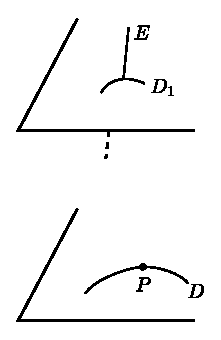
\includegraphics{figure/fig1.eps}

\medskip
{\bf Fig 1.}
\end{figure}
\end{minipage}
\qquad
\begin{minipage}[b]{5cm}
\begin{figure}[H]
\centering
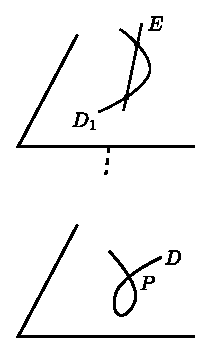
\includegraphics{figure/fig2.eps}

\medskip
{\bf Fig 2.}
\end{figure}
\end{minipage}

\bigskip

\begin{minipage}[b]{5cm}
\begin{figure}[H]
\centering
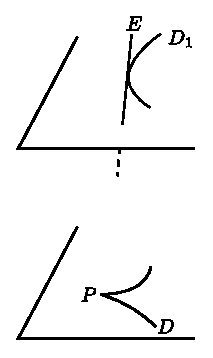
\includegraphics{figure/fig3.eps}

\medskip
{\bf Fig 3.}
\end{figure}
\end{minipage}
\qquad
\begin{minipage}[b]{5cm}
\begin{figure}[H]
\centering
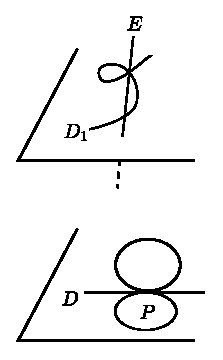
\includegraphics{figure/fig4.eps}

\medskip
{\bf Fig 4.}
\end{figure}
\end{minipage}
\end{center}
\end{REM*}

\section{Conductor}\label{chap2:sec5}
 Let\pageoriginale $\varphi :X\to
Y$ be any morphism. We define the conductor $\underline{f}$ of this
morphism as the $O_Y$-module,
$$
\underline{f} = \Hom_{O_Y}(\varphi_*O_X,O_Y)
$$
We note that when $\varphi$ is birational,
$$
\underline{f}= Ann(\varphi_*O_X/_{O_X})
$$
In case $\omega_Y$ is a line bundle, we see that,
\begin{align*}
\underline{f} &=\Hom_{O_Y}(\varphi_*O_X,O_Y)\\
&= \Hom_{O_Y}(\varphi_*O_X,\omega_Y)\underset{O_Y}{\otimes}
\omega_Y^{-1}\\
&= \varphi_*\omega_X\underset{O_Y}{\otimes}\omega_Y^{-1}
\end{align*}
So going back to our case, let $X$ be a non-singular irreducible
surface. Let $D$ be a reduced and irreducible curve on $X$. Let $P$ be
a point on $X$ and $X_1$, the blown up of $X$ at $P$ and $\varphi:X_1
\longrightarrow X$ the canonical map. Let $D_1$ be the proper
transform of $D$. We denote restriction of $\varphi$ to $D_1$ also by
$\varphi$. Let $E$ be the exceptional divisor and $r=m_P(D)$. So we
have $\varphi:D_1\longrightarrow D$ is a finite birational map and
$\omega_D$ (the dualising sheaf of $D$) is a line bundle. Let
$\underline{f}$ be the conductor of $\varphi$. Then we have 
$$
\underline{f}=\varphi_*\omega_{D_1}\otimes_{O_D}\omega_D^{-1}
$$
Now, if $\omega_{X_1}$, is the dualising sheaf of $X_1, \omega_{D_1}=
O_{X_1}(D_1)\underset{O_{X_1}}{\otimes}\omega_{X_1} \underset{O_{X_1}}
{\otimes}O_{D_1}$ because $D_1$ is a divisor on $X_1$. So
\begin{align*}
\omega_{D_1} &= O_{X_1}(\omega^*D-rE)\underset{O_{X_1}}{\otimes}
\varphi^*\omega_X\underset{O_{X_1}}{\otimes}O_{X_1}(E)
\underset{O_{X_1}}{\otimes}O_{D_1}\\
&= \varphi^*(O_{X}(D))\underset{O_{X_1}}{\otimes}O_{X_1}(-(r-1)E)
\underset{O_{X_1}}{\otimes}\varphi^*\omega_X
\underset{O_{X_1}}{\otimes}O_{D_1}
\end{align*}\pageoriginale
where $\omega_X$ is the dualising sheaf on $X$. Since
$O_{D_1}= \varphi^*(O_D)\underset{O_{X_1}}{\otimes}O_{D_1}$ we have, 
\begin{align*}
\omega_{D_1} &= \varphi^*(O_X(D)\underset{O_{X}}{\otimes}\omega_X)
\underset{O_{X_1}}{\otimes}O_{X_1}(-(r-1)E)\underset{O_{X_1}}{\otimes}
\varphi O_D\underset{O_{X_1}}{\otimes}O_{D_1}\\
&= \varphi^*(O_X(D)\underset{O_X}{\otimes}\omega_X\otimes O_D)
\underset{O_{X_1}}{\otimes}O_{X_1}(-(r-1)E)\otimes O_{D_1}\\
&= \varphi^*\omega_D\underset{O_{D_1}}{\otimes}O_{D_1}(-(r-1)E).\\
\omega_{D_1} &= \varphi^*\omega_D\underset{O_{D_1}}{\otimes} O_{D_1} (-(r-1)E
\end{align*}

\begin{claim*}
$$
\underline{f}=\varphi_*(O_{D_1}(-(r-1)E)).
$$

We have a canonical injection,
$$
0\longrightarrow O_{D_1}(-(r-1)E)\longrightarrow O_{D_1}
$$
This gives two injections of $O_D$-modules,
\begin{align*}
&0\longrightarrow\varphi_*O_{D_1}(-(r-1)E)\underset{O_D}{\otimes}
\omega_D\longrightarrow\varphi_*O_{D_1}\underset{O_D}{\otimes}\omega_D\\
\intertext{and}
&0\longrightarrow\varphi_*(O_{D_1}(-(r-1)E)\underset{O_{D_1}}{\otimes}
\varphi^*\omega_D)\longrightarrow\varphi_*\varphi^*\omega_D
\end{align*}
\end{claim*}

We\pageoriginale have a canonical $O_D$-module homomorphism $\omega_D
\longrightarrow\varphi_*\varphi^*\omega_D$ which in turn gives a
$\varphi_*O_{D_1}$ homomorphism,
$$
\omega_D\underset{O_D}{\otimes}\varphi_*O_{D_1}\longrightarrow\varphi_*
\varphi^*\omega_D\underset{O_D}{\otimes}\varphi_*O_{D_1}
$$
Since $\varphi_*\varphi^*\omega_D$ is a $\varphi_*O_{D_1}$-module we
have a canonical $\varphi_*O_{D_1}$ - homomorphism
$$
\varphi_*\varphi^*\omega_D\underset{O_D}{\otimes}\varphi_*O_{D_1}
\longrightarrow\varphi_*\varphi^*\omega_D
$$
The composite gives us a canonical homomorphism,
$$
\omega_D\underset{O_D}{\otimes}\varphi_*O_{D_1}\longrightarrow
\varphi_*\varphi^*\omega_D.
$$

Since $\varphi$ is an affine morphism, this is an isomorphism. So we
have a diagram:
\[
\xymatrix{
0\ar[r] & \varphi_*O_{D_1}(-(r-1)E)\underset{O_D}{\otimes} \omega_D
\ar[rr]\ar[d] & &
\varphi_*O_{D_1}\underset{O_D}{\otimes}\omega_D\ar[d]^{\wr}\\
0\ar[r] & \varphi_*\omega_{D_1}\ar[r] & & \varphi_*\varphi^*\omega_D 
}
\]

Since $\varphi$ is affine, one sees that
$\varphi_*O_{D_1}(-(r-1)E) \underset{O_D}{\otimes}\omega_D$ and
$\varphi_*\omega_{D_1}$ coincide locally and hence globally. \ie
$$
\varphi_*O_{D_1}(-(r-1)E)\underset{O_D}{\otimes}\omega_D=\varphi_*\omega_{D_1}.
$$

So
$$
\underline{f}=\varphi_*\omega_{D_1}\underset{O_D}{\otimes}\omega_D^{-1},
\underline{f}=\varphi_*O_{D_1}(-(r-1)E).
$$

From\pageoriginale this formula we get,
$$
\ell(\varphi_*O_{D_1}/\underline{f})=\ell(\varphi_*
O_{D_1})/_{\varphi_*O_{D_1}(-(r-1)E)}). 
$$

We have an exact sequence,
$$
0\longrightarrow O_{D_1}(-(r-1)E)\longrightarrow O_{D_1}\longrightarrow
O_{{D_1}/O_{D_1}(-r-1)E)} \longrightarrow 0.
$$

Since $\varphi$ is affine, $\varphi_*$ is an exact functor. So we
have,
$$
0\longrightarrow\varphi_*O_{D_1}(-(r-1)E)\longrightarrow\varphi_*O_{D_1}
\longrightarrow\varphi_*(O_{D_1}/O_{D_1}(-(r-1)E))\longrightarrow 0
$$
\ie
\begin{align*}
\varphi_*O_{D_1/\varphi_*O_{D_1}}(-(r-1)E) &=
\varphi_*(O_{D_1}/O_{D_1}(-(r-1)E))\\
\ell(\varphi_*O_{D_1/\underline{f}}) &= \ell
(\varphi_*(O_{D_1}/O_{D_1}(-(r-1)E))\\
&= \dim_KH^\circ(D,\varphi_*(O_{D_1}/O_{D_1}(-(r-1)E))\\
&= \dim_kH^\circ(D_1,O_{D_1}/O_{D_1}(-(r-1)E))\\
&= \deg O_{D_1}((r-1)E)\\
&= (r-1).d^\circ O_{D_1}(E)\\
&= r(r-1).
\end{align*}

This gives a cohomology exact sequence
\begin{align*}
0\longrightarrow H^\circ(D,\varphi_*\omega_{D_1}) &\longrightarrow
H^\circ(D<\omega_D)\longrightarrow H^\circ(D,O_{D/\underline{f}})\\
&\longrightarrow H^1(D,\varphi_*\omega_{D_1})\longrightarrow H^1(D,
\omega_D)\longrightarrow 0
\end{align*}
Since\pageoriginale $\varphi$ is affine,
$H^1(D,\varphi_*\omega_{D_1})=H^1(D_1,\omega_{D_1})$, and by duality,
$H^1(D_1,\break\omega_{D_1})=H^\circ(D_1, O_{D_1}^\nu)$ and
$H^1(D,\omega_D)=H^\circ(D, O_D^\nu)$. So we get an exact sequence
\begin{align*}
0 &\longrightarrow H^\circ(D_1,\omega_{D_1})\longrightarrow H^\circ(D,
\omega_D)\longrightarrow H^\circ(D, O_{D/\underline{f}})\\
&\longrightarrow H^\circ(D_1,O_{D_1}^\nu)\longrightarrow H^\circ(D,
O_D^\nu)\longrightarrow 0
\end{align*}
Since $D$ and $D_1$ are reduced and irreducible, the last
two terms are one dimensional over $k$ and hence isomorphic. Therefore
we have an exact sequence,
$$
0 \longrightarrow H^\circ(D_1,\omega_{D_1})\longrightarrow H^\circ(D,
\omega_D) \longrightarrow H^\circ(D,
O_{D/\underline{f}})\longrightarrow 0
$$

\subsection[Gorenstein Theorem]{Gorenstein Theorem for the Blowing
  up}\label{chap2:ssec5.1}

 Let the situation be as before.

\begin{THM*}
(local Gorenstein theorem for a blowing up). Let $D$ be a reduced
  irreducible divisor on a regular projective surface over an
  algebraically closed field. Let $D_1$ be the blowing up of $D$ at a
  closed point, then:
$$
2.\ell(\varphi_*O_{D_1}/O_D)=2.\ell(O_{D/\underline{f}})=\ell(\varphi_*
O_{D_1/\underline{f}}).
$$
\end{THM*} 

\begin{proof}
We will prove the first equality. The second equality follows because
$$
\ell(\varphi_*O_{D_1/\underline{f}})=\ell(\varphi_*O_{D_1}/O_D)+\ell 
(O_{D/\underline{f}}).
$$

We have an exact sequence,
$$
0\longrightarrow\underline{f}\longrightarrow O_D\longrightarrow
O_{D/\underline{f}}\longrightarrow 0,
$$
which\pageoriginale gives after tensoring by $\varphi_D$, an exact
sequence, 
$$
0\longrightarrow \underline{f}\underset{O_D}{\otimes}\omega_D
\longrightarrow \omega_D \longrightarrow O_{D/\underline{f}}
\longrightarrow 0.
$$

Since $\underline{f}\otimes\omega_D^.=\varphi_*\omega_{D_1}$ we have
an exact sequence,
$$
0\longrightarrow\varphi_*\omega_{D_1} \longrightarrow\omega_D
\longrightarrow O_{D/\underline{f}}\longrightarrow 0.
$$

Therefore
\begin{equation*}\label{chap2:eqA}
\ell(O_{D/\underline{f}})=\dim H^\circ(D,\omega_D)-\dim H^\circ
(D_1,\omega_{D_1})\tag{A}  
\end{equation*} 
Again we  have an exact sequence,
$$
0\longrightarrow O_D \longrightarrow\varphi_*O_{D_1}\longrightarrow
\varphi_* O_{D_1}/O_D\longrightarrow 0
$$
which gives a cohomology exact sequence,
\begin{equation*}
\begin{split}
0\longrightarrow H^\circ(D,O_D)\longrightarrow H^\circ(D_1,O_{D_1})
\longrightarrow H^\circ(D,\varphi_*O_{D_1}/O_D)\\
H^\circ(D,\omega_D^\nu)\longrightarrow H^\circ(D_1,\omega_{D_1}^\nu)
\longrightarrow 0.
\end{split}
\end{equation*}

Further the first two terms are one-dimensional and hence isomorphic
to each other. So we have,
$$
0 \longrightarrow H^\circ(D,\varphi_*O_{D_1}/O_D)\longrightarrow
H^\circ(D,\omega_D^\nu)\longrightarrow H^\circ(D_1,\omega_{D_1}^\nu)
\longrightarrow 0
$$
is exact. Therefore 
\begin{equation*}\label{chap2:eqB}
\ell(\varphi_*O_{D_1}/O_D)=\dim H^\circ(D,\omega_D)-\dim H^\circ
(D_1,\omega_{D_1}).\tag{B}
\end{equation*}

Using\pageoriginale \eqref{chap2:eqA} and \eqref{chap2:eqB} we get 
$$
\ell(O_{D/\underline{f}})=\ell(\varphi_*O_{D_1/O_D}).
$$
\end{proof}

\begin{Coro*}
Let $\overline{M}$ be the sheaf of ideals of $O_D$ defining $P$. Then 
$$
\underline{f}=\overline{M}^{r-1}.
$$
\end{Coro*}

\begin{proof}
We have a map $\varphi^*\overline{M}^j\longrightarrow O_{D_1}$ for
every $j$ and the image of the map is $O_{D_1}(-jE)$. So we have a map
$\varphi_* \varphi^*\overline{M}^{r-1}\longrightarrow\varphi_* O_{D_1}
(-(r-1)E)$. But $\varphi_*O_{D_1}(-(r-1)E)=\underline{f}$ and is an
ideal in $O_D$. So we have the map $\varphi_*\varphi^*
\overline{M}^{r-1}\longrightarrow\underline{f}\subset O_D$. The map
$\overline{M}^{r-1}\subset O_D$ is canonical and hence
$\overline{M}^{r-1}\longrightarrow\underline{f}$ is an inclusion. But
by the Gorenstein theorem,
$$
\ell(O_D/_{\underline{f}})=\frac{r(r-1)}{2}
$$
and by the computation of the Hilbert-Samuel function,
$$
\ell(O_D/_{\overline{M}^{r-1}})=\frac{r(r-1)}{2}.
$$

This implies that $\overline{M}^{r-1}=\underline{f}$.
\end{proof}

\begin{REM*}
By the above corollary, $D_1$ is also the blowing up of
$\underline{f}$. 
\end{REM*}

\section[Resolution of Singularities..]{Resolution of Singularities of
  a  Reduced\hfil\break Irreducible Curve on a Non-Singular
  Surface}\label{chap2:sec6} Let $D$ be a reduced irreducible curve on
a non-singular surface $X$ and $P$ be any point on $X$. Let $X_1$ be
the blown up of $X$ at $P$ and $D_1$, the proper transform of $D$.
\begin{align*}
\varphi &:X_1\longrightarrow X\\
\varphi &:D_1\longrightarrow D
\end{align*}

\begin{claim*}
The\pageoriginale canonical morphism,
$O_D\longrightarrow\varphi_*O_{D_1}$ is an isomorphism if and only if
either $D$ is non-singular at $P$ or $D$ does not pass through $P$.
\end{claim*}

The homomorphism $O_D\longrightarrow\varphi_*O_{D_1}$ is an
isomorphism if and only if $\ell(\varphi_*O_{D_1}/O_D)=0$. The
condition $\ell(\varphi_*O_{D_1}/O_D)=0$ is equivalent to
$\frac{r(r-1)}{2}=0$, where $r=m_P(D)$. This is equivalent to $r=0$ or
$r=1$, \ie either $D$ does not pass through $P$ or $D$ is non-singular
at $P$.

Let $D$ be any reduced irreducibel curve on a regular surface
$X$. Suppose that the normalisation $\bar{D}$ of $D$ is finite over
$D$. If $P$ is a point on $D$ where $D$ is singular, we blow up $X$ at
$P$ and let $X_1$ be the blown up of $X$ and $D_1$ the proper
transform of $D$. Again if $Q$ is a singular point on $D_1$ we blow up
$X_1$ at $Q$ and let $X_2$ be the blow up of $X_1$ and $D_2$, the
proper transform of $D_1$. We can continue this process to get a chain,
$$
D_s\xrightarrow{\varphi_s}D_{s-1}\longrightarrow D_2
\xrightarrow{\varphi_2}D_1\xrightarrow{\varphi_1}D.
$$

Since all these maps are finite and birational, we have a map $\bar{D}
\longrightarrow D_s$ where $\bar{D}$ is the normalisation of $D$. It
is clear that this process stops because the length $\varphi_*
O_{\bar{D}}/O_{D_s}$ decreases and is bounded by the length of
$\varphi_* O_{D}/O_D$
\begin{Examples*}
\begin{itemize}
\item [(1)] Consider the curve $C$ given by $Y^nZ-X^{n+1}$ in
$\mathbb{P}^2$, where $(X, Y, Z)$ are the homogeneous
coordinates. $P=(0,0,1)$ is the only singular point of $C$. If $C$
is the normalisation of $C$, one easily sees that,
$\ell(\varphi_*O_{C}/O_C)$ is equal to $\frac{n(n-1)}{2}.m_P(C)=n$
and so if we blow up $C$ at $P$ to get\pageoriginale a curve $C_1$, we
get $\ell(\varphi_*O_{C_1}/O_C)=\frac{n(n-1)}{2}$ So $C_1$ is
isomorphic to $\bar{C} \ie C$ gets desingularised in one blowing
up. (\cf Fig. 3)

\item [(2)] Take a curve with ordinary singularities, \ie each branch
  at any point is non-singular and it has distinct tangents for each
  branch. Since in the blowing up the number of points on the
  exceptional divisor corresponds to these tangents, the curve is
  non-singular at those points. So be blowing up the singular points
  once we get the desingularisation (\cf Fig. 2)  
\end{itemize}
\end{Examples*}

Now we will calculate the conductor of $D_i$ over $D$ in terms of the
relative conductors. Let $\underline{f}$ be the conductor of the map
$D_i\xrightarrow{\varphi_1\circ\ldots\circ\varphi_i}D$ and
$\underline{f}_j$ the conductor of the map $D_j\longrightarrow
D_{j-1}$ Then we claim:
$$
\underline{f}=\underline{f}_1.\varphi_{1^*}\underline{f}_2.(\varphi_1
\circ\varphi_2)_*\underline{f}_3\ldots(\varphi_1\circ\varphi_2\ldots\circ
\varphi_{i-1})_*\underline{f}_1.
$$

There is a canonical inclusion of the ideal sheaf on the right hand
side into the ideal sheaf $\underline{f}$. So to prove equality one
only has to show it locally.

So we have a sequence of semilocal rings. $A_\circ\subset A_1\subset
A_2 \subset\ldots\subset A_i$ the corresponding morphism of $\Spec
A_j$'s are finite and birational. Let the same letters denote the
conductors. We have $\underline{f}_1.\underline{f}_2\ldots
\underline{f}_i\subset\underline{f}.\underline{f}$ is an ideal of
$A_\circ$. Let $a\in\underline{f}$. So $a.A_i\subset A_\circ$. 

Since $A_i$'s are semilocal, relative conductors are principal above,
\ie $\underline{f}_j=t_jA_j$ where $t_{j^.}$ belongs to
$\underline{f}_j$

We will show that $at_1^{-1}$ is an element of the relative conductor
of $A_1\subset A_i$ and by induction we will be through. We therefore
want to show that $aA_i\subset t_1A_1$.\pageoriginale Since
$A_1\subset A_i$ and $aA_i\subset A_\circ$, we see that any element of
a $A_i$ annihilates $A_1/{A_\circ}$ and hence $aA_i\subset t_1A_1=
\underline{f}_1.\, \ie\, at_1^{-1}.A_i\subset A_1$. So by induction we see
that $at_1^{-1}.t_2^{-1}\ldots t_{i-1}^{-1}. A_i\subset A_{i-1}\,\ie\,
at_1^{-1} t_2^{-1}\ldots t_{i-1}^{-1}$ belongs to $\underline{f}_i$,
which implies 
\begin{align*}
& a\quad\text{belongs to}\quad\underline{f}_1\ldots\underline{f}_1\\
& \ie\,\underline{f}=\underline{f}_1\ldots\underline{f}_i.
\end{align*}

\begin{REM*}
$D_i$ can also be obtained by blowing up $D$ at the conductor on the
  map $D_i\longrightarrow D$.
\end{REM*}

\begin{def*}
Let $D$ be a reduced irreducible curve. The set of infinitely near
points of $D$ is equal to the disjoint union of closed points of
curves $D$ which can be obtained from $D$ by a finite sequence of
blowing-ups of closed points.
\end{def*}

\section{Adjoint Systems}\label{chap2:sec7} Let $X$ be a non-singular
surface, $L$ a line bundle on $X$. Let $D$ be a reduced irreducible
curve on $X$. Let $\bar{D}$ be its normalisation. Let $\underline{f}$
be the conductor of the map $\bar{D}\longrightarrow D$. So that
$\underline{f}$ is an ideal sheaf in $O_D$. Since there is a
surjection $O_X\longrightarrow O_D$, there exists a unique ideal sheaf
$\underline{F}$ in $O_X$ such that $O_{X/\underline{F}}=O_{D/
\underline{f}}$. ($\underline{F}$ is the inverse image of
$\underline{f}$ in $O_X$).
\begin{def*}
Let $L$ be a line bundle on $X$. An effective divisor $D_1$ on $X$ is
an {\it adjoint of type $L$} with respect to $D$ if $O_X(D_1)=L$ and
the corresponding element in $H^\circ(X,L)$ is in the sublinear system
$H^\circ(X,\underline{F}\otimes L)$. 
\end{def*}

\begin{Prop*}
Let $X$ be a regular surface and $D$, a reduced irreducible divisor on
$X$. Suppose that the normalisation $\bar{D}$ of $D$ is finite over
$D$. A divisor\pageoriginale $D'$ on $X$ is an adjoint of $D$ of type
$L$ if and only if the following conditions are satisfied. 
\begin{itemize}
\item [i)] $O_X(D')=L$
\item [ii)] For any finite chain of blowing-ups of closed points,
$$
X_s\longrightarrow X_{s-1}\longrightarrow\ldots\longrightarrow X_1
\longrightarrow X_\circ=X,
$$
\end{itemize}
if we denote by $f_{s,j}$ the morphism from $X_s$ to $X_j(j<s)$ then
for any point $Q$ in $X_s$,
$$
m_Q(f_{s,\circ}^*D'+f_{s,1}^*E_1+\cdots +f_{s,s-1}^*E_{s-1}+E_s)\geq
m_Q(f_{s,\circ}^*D)-1
$$
where $(*)$ denotes the total transform and $E_j$, the last
exceptional divisor of $X_j$. 
\end{Prop*}

The proof is simple and is carried out by induction on $s$.
\begin{REMS*}
\begin{enumerate}
\item If $D'$ satisfies the property that 
$$
m_Q(D'_s)\geq m_Q(D_s)-1,
$$
where $D_s$ and $D'_s$ are proper transforms of $D$ and $D'$ in $X_s$,
then $D'$ is an adjoint of $D$. This can be easily seen by showing
that this condition is stronger than the condition in the Proposition.
\item If all singularities of $D$ become desingularized at the first
blowing up, then the two conditions are actually equivalent. 
\end{enumerate}
\end{REMS*}

\begin{exam}\label{chap2:exm1}
Polar Curves.
\begin{figure}[H]
\centering
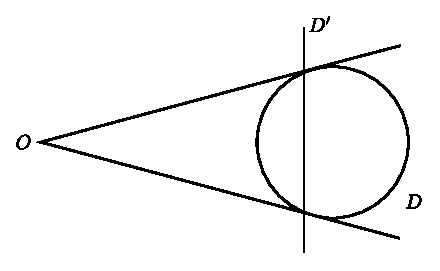
\includegraphics{figure/fig5.eps}
\end{figure}

Let\pageoriginale $D$ be a projective plane integral curve of
characteristic zero. Let $0$ be a point in the plane with homogeneous
co-ordinates $a_0,a_1,a_2$. If $F$ is the homogeneous equation of $D$
the polar curve $D'$ of $D$ with respect to $0$ is the curve with the
equation $\sum a_i\frac{\partial F}{\partial X_i}$ The polar curve
is an adjoint of type $O_{\mathbb{P}^2}(m-1)$ where $m$ is the degree
of $D$.
\end{exam}

\begin{exam}\label{chap2:exm2}
Suppose that $D$ has only ordinary double points as
singularities. Then a curve $D'$ is an adjoint of $D$ if and only if it
passes through all singular points of $D$.
\begin{figure}[H]
\centering
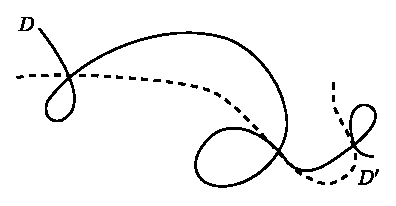
\includegraphics{figure/fig6.eps}
\end{figure}
\end{exam}

\begin{exer*}
(Max\pageoriginale Noether theorem: $AF+BG$). Let $F$ and $G$ be
  homogeneous polynomials defining two curves $(F)$ and $(G)$ in
  $\mathbb{P}^2$. Suppose that $(F)$ is reduced and irreducible and is
  not a component of $(G)$. Then a homogeneous polynomial $H$ is of
  the form $AF+BG$, where $A$ and $B$ are polynomials, if for any
  infinitely near point $Q$ of $(F), m_Q(F.H)\geq m_Q(F.G)$.  
\end{exer*}

(Hint:Prove that there exists such a $B$ which defines an adjoint
curve of $(F)$)

\section{Gorenstein Theorem}\label{chap2:sec8}
\begin{THM*}
Let $C$ be an integral curve in $\mathbb{P}^2$ of degree $m$. Then the
adjoint curves of $C$ of type $O_{\mathbb{P}^2}(m-3)$ cut out on $C$,
the complete canonical system of $\bar{C}$, where $\bar{C}$ is the
normalisation of $C$.
\end{THM*}

\begin{proof}
Let $\underline{f}$ be the conductor of $\bar{C}\longrightarrow C$ and
$\underline{F}$ the inverse image of $\underline{f}$ under the map
$O_{\mathbb{P}^2}\longrightarrow O_C$. Then by the previous
proposition we know that the adjoints of type $O_{\mathbb{P}^2}(m-3)$
are zeros of section of $\underline{F}(m-3)$. So the theorem states
that the image of $H^\circ(\mathbb{P}^2,\underline{F}(m-3))
\longrightarrow H^\circ(C,\omega_C)$ under the canonical map is equal
to the image of $H^\circ(\bar{C},\omega_{\bar{C}})$ in $H^\circ(C,
\omega_C)$. 

We have a commuting diagram of exact sequences as follows:
\[
\xymatrix{
& 0\ar[d] & 0\ar [d]& & \\
& O_{\mathbb{P}^2}(-m)\ar[d]\ar@{}[r]|{=}& O_{\mathbb{P}^2}(-m)
\ar[d] & &\\ 
0 \ar[r] & F \ar[d] \ar[r] & O_{\mathbb{P}^2} \ar[d] \ar[r] &
O_{C/_{\underline{f}}}\ar @{}[d]|{\|} \ar[r] & 0\\
0 \ar[r] & \underline{f} \ar[d] \ar[r] & O_C \ar[d] \ar[r] &
O_{C/_{\underline{f}}} \ar[r] & 0\\
& 0 & 0 & &
}
\]

Tensoring\pageoriginale the diagram by $O_{\mathbb{P}^2}(m-3)$ we get
a commutative diagram of exact sequences:
\[
\xymatrix{
& 0 \ar[d] & 0 \ar[d] & &\\
& O_{\mathbb{P}^2}(-3) \ar @{} [r] |{=} \ar[d]& O_{\mathbb{P}^2}(-3) \ar[d]
& &\\
0 \ar[r] & \underline{F}(m-3) \ar[d] \ar[r] & O_{\mathbb{P}^2}(m-3)
\ar[d] \ar[r] & O_{C/_{\underline{f}}} \ar[r] \ar @{} [d]|{\|} & 0\\
0 \ar[r] & \underline{f}(m-3) \ar[d] \ar[r] & O_C(m-3) \ar[d] \ar[r] &
O_{C/_{\underline{f}}} \ar[r] & 0\\
& 0 & 0 & &
}
\]

Since $C$ is a divisor on $\mathbb{P}^2$,
\begin{align*}
\omega_C &= (O_{\mathbb{P}^2}(m)\otimes O_{\mathbb{P}^2}(-3))/O_C\\
&= O_C(m-3)
\end{align*}
Again $\varphi_*\omega_{\bar{C}}=\omega_C\otimes\underline{f}=
\underline{f}(m-3)$. So we have a diagram:
\[
\xymatrix{
& 0 \ar[d] &  0 \ar[d]\\
& O_{\mathbb{P}^2}(-3) \ar[d] \ar @{} [r] |{=} & O_{\mathbb{P}^2}(-3)
\ar[d]\\
0 \ar[r] & \underline{F}(m-3) \ar[d] \ar[r] & O_{\mathbb{P}^2}(m-3)
\ar[d]\\ 
0 \ar[r] & \varphi_*\omega_{\bar{C}} \ar[d] \ar[r] & O_C(m-3)=\omega_C
\ar[d]\\
& 0 & 0   
}
\]
Thus\pageoriginale we get a diagram of exact sequences:
\[
\xymatrix{
0 \ar[r] & H^\circ(\mathbb{P}^2,\underline{F}(m-3)) \ar[d] \ar[r] &
H^\circ(\mathbb{P}^2, O_{\mathbb{P}^2}(m-3)) \ar[d]\\
0 \ar[r] & H^\circ(C,\varphi_*\omega_{\bar{C}}) \ar[d] \ar[r] &
H^\circ(C,\omega_C)\\ 
& H^1(\mathbb{P}^2, O_{\mathbb{P}^2}(-3)) & 
}
\]
Since $H^1(\mathbb{P}^2,O_{\mathbb{P}^2}(-3))=0$, the map
$$
H^\circ(\mathbb{P}^2,\underline{F}(m-3))\longrightarrow H^\circ(C,
\varphi_*\omega_{\bar{C}})=H^\circ(\bar{C},\omega_{\bar{C}})
$$
is a surjection, which proves the theorem.
\end{proof}

\section{Regularity of the Adjoint System}\label{chap2:sec9} Let $C$
be an integral curve on a smooth projective surface $X$ over an
algebraically closed field. Let $\bar{C}$ be the normalisation of $C$
and $\underline{f}$ the conductor. Let $\underline{F}$ be the inverse
image of $\underline{f}$ under the map $O_X\longrightarrow O_C$. So we
have a map $\underline{F}\longrightarrow O_C$. Therefore we have a
map,
$$
\underline{F}\otimes O_X(C)\otimes\omega_X\longrightarrow O_C\otimes
O_X(C)\otimes\omega_X=\omega_C,
$$
which in turn gives a map,
$$
H^\circ(X,\underline{F}\otimes\omega_X(C))\longrightarrow H^\circ(C,
\omega_C).
$$

Let $V$ be the image of this map. We denote by $q$ the irregularity of
$X$:
$$
q=\dim H^1(X, O_X)=\dim H^1(X,\omega_X).
$$
\begin{def*}
The adjoint system is called regular if 
$$
\dim H^\circ(\bar{C},\omega_{\bar{C}})-\dim V=q.
$$
\end{def*}

\begin{Prop*}
If\pageoriginale the adjoint system of $C$ is regular then $H^1(X,\break O_X
(-C))=0$.
\end{Prop*}

\begin{proof}
We have commutative diagram of exact sequences
\[
\xymatrix{
& 0 \ar[d] & 0 \ar[d] & &\\
& O_X(-C) \ar[d] \ar @{} [r] |{=} & O_X(-C) \ar[d] & &\\
0 \ar[r] & \underline{F} \ar[d] \ar[r] & O_X \ar[d] \ar[r] &
O_{C/_{\underline{f}}} \ar[r] & 0\\
0 \ar[r] & \underline{f} \ar[d] \ar[r] & O_C \ar[d] \ar[r] &
O_{C/_{\underline{f}}} \ar[r] & 0\\
& 0 & 0 & & 
}
\] 
which gives a commutative diagram of exact sequences, by tensoring
with $\omega_X(C)$.
\[
\xymatrix{
& 0 \ar[d] & 0 \ar[d]\\
& \omega_X \ar[d] \ar @{} [r] |{=} & \omega_X \ar[d] & &\\
0 \ar[r] & \underline{F}\otimes\omega_X(C) \ar[d] \ar[r] & \omega_X(C)
\ar[d] \ar[r] & O_{C/_{\underline{f}}} \ar[r] & 0\\
0 \ar[r] & \underline{f}\otimes\omega_C \ar[d] \ar[r] & \omega_C
\ar[d] \ar[r] & O_{C/_{\underline{f}}} \ar[r] & 0\\
& 0 & 0 & &
}
\]
Taking cohomologies we have the following diagram of exact
sequen\-ces:
\newpage

\[
\xymatrix{
& 0 \ar[d] & 0 \ar[d]\\
& H^\circ(X,\omega_X) \ar[d] \ar @{} [r] |{=} & H^\circ(X,\omega_X)
\ar[d]\\
0 & H^\circ(\underline{F}\otimes\omega_X(C)) \ar[d] \ar[r] &
H^\circ(X,\omega_X(C)) \ar[d]\\
0 & H^\circ(\bar{C},\omega_{\bar{C}}) \ar[d] \ar[r] & H^\circ(C,
\omega_C) \ar[d]\\
& H^1(X,\omega_X) \ar @{} [r] |{=} & H^1(X,\omega_X) \ar[d]\\
& & H^1(X,\omega_X(C)) \ar[d]\\
& & H^1(C,\omega_C) \ar[d]\\
& & H^2(X,\omega_X)) \ar[d]\\
& & H^2(X,\omega_X(C)) \ar[d]\\
& & 0 
}
\]\pageoriginale

First $H^2(X,\omega_X(C))=H^\circ(X,O_X(-C))=0$. Again $H^1(C,
\omega_C^\nu)=H^\circ(C,O_C)=k$ and
$H^2(X,\omega_X^\nu)=H^\circ(X,O_X)=k$, and since the map $H^1(C,
\omega_C)\longrightarrow H^2(X,\omega_X)$ is a surjection it must be
an isomorphism. So the map $H^1(X,\omega_X)\longrightarrow H^1(X,
\omega_X(C))$ is surjection.

The regularity of the adjoint system implies that the map
$H^\circ(\bar{C},\break\omega_{\bar{C}})\longrightarrow H^1(X,\omega_X)$ is
surjective. So we see that the map $H^\circ(C,\omega_C)
\longrightarrow, H^1(X,\omega_X)$ is surjective. The exactness of the
sequence implies that $H^1(X,\omega_X(C))=0$, \ie
$$
H^1(X,O_X(-C))=0.
$$ 

There\pageoriginale are much stronger results in this direction in
characteristic zero by Kodaira \cite{key2} and others. 
\end{proof}

\begin{THM*}
{\bf (Kodaira).} Let $X$ be a K\"ahlarian variety, $L$ an ample line
bundle on $X$. Then $H^i(X;L^{-1})=0$ for $i=0, 1,\ldots\dim X-1$.

The reader can find similar results and an introduction to the above
theorem in $D$. Mumford \cite{key3}. There are several results in this
direction, for \eg see \cite{key1}, \cite{key4}, \cite{key5}, \cite{key6}
and \cite{key7}. But note that all these results are for
characteristic zero.
\end{THM*}

\section[A Difference Between]{A Difference Between Characteristic
  Zero and Characteristic $p$}\label{chap2:sec10} In this section, as
before, $X$ is a smooth connected surface, projective over a field
$k, \,C$ a reduced irreducible curve on $X,\bar{C}$, the normalisation
of $C$ and $\bar{X}$, the surface obtained after a finite number of
dilations of points from $X$, such that the proper transform of $C$ on
$X$ is $\bar{C}$. We will denote by $\underline{F}$, the sheaf of
adjoint curves to $C$.
\begin{Prop*}
Let $X'\longrightarrow X$ be the blowing up of a closed point $P$ of
$X, C'$, the proper transform of $C,\underline{F}'$, the sheaf of
adjoint curves to $C$. There is a canonical isomorphism,
$$
H^1(X',\underline{F}'\otimes\omega_X(C'))\longrightarrow H^1(X,
\underline{F}\otimes\omega_X(C)).
$$

In other words, $H^1(X,\underline{F}\otimes.\omega_X(C))$ is a
birational invariant (equal to $H^1(\bar{X},\omega_{\bar{X}}(\bar{C}))
\simeq H^1(\bar{X}, O_{\bar{X}}(-C))$. 
\end{Prop*}

\begin{proof}
Let $M$ be the sheaf of ideals defining $P$ in $X$ and $r$, the
multiplicity of $C$ at $P$. By the Leray spectral sequence for the
morphism, $g:X'\longrightarrow X$,\pageoriginale it will be enough to
prove that 
\begin{align*}
& g_*(\underline{F}'\otimes\omega_{X'}(C'))=\underline{F}\otimes
\omega_X (C)\tag{i}\label{chap2:eqi}\\
\intertext{and} 
&R^1g_*(\underline{F}'\otimes\omega_{X'}(C')) =
0\tag{ii}\label{chap2:eqii}
\end{align*}

We know that, $\omega_{X'}=g^*\omega_X\otimes O_{X'}(E)$, where $E$ is
the exceptional divisor.
$$
O_{X'}(C')=g^*O_X(C)\otimes O_{X'}(-rE).
$$

So to prove \eqref{chap2:eqii}, it is enough to have
\begin{equation*}
R^1g_*(\underline{F}'\otimes O_{X'}(-(r-1)E))=0\tag{ii}
\end{equation*}

If $\underline{f}'$ is the conductor of $C'$, one has the exact
sequence,
$$
0\longrightarrow O_{X'}(-C')\longrightarrow\underline{F}'
\longrightarrow\underline{f}'\longrightarrow 0
$$
Tensoring this by $O_{X'}(-(r-1)E)$, one gets
\begin{align*}
0&\longrightarrow O_{X'}(-C'-(r-1)E)\longrightarrow\underline{F}'
\otimes O_{X'}(-(r-1)E)\\
&\longrightarrow\underline{f}'\otimes O_{X'}
(-(r-1)E)\longrightarrow 0\tag{*}\label{chap2:eq*}
\end{align*}
to be exact. Since the morphism $C'\longrightarrow C$ is affine, from
the long exact sequence for derived functors, we see that it is
sufficient to prove,
\begin{equation*}
R^1g_*(O_{X'}(-C'-(r-1)E))=0\tag{iii}\label{chap2:eqiii}
\end{equation*}
But $R^1g_*$ commutes with base change, since it is the last non-zero
cohomology functor. So it will be enough to prove that,
$$
O_{X'}(-C'-(r-1)E)_{/E}\simeq O_{\mathbb{P}^1}(-1).
$$

This is evident, because $C'/E$ is equal to $r$ points counted with
multiplicity and hence $O_{X'}(-C')/E=O_{\mathbb{P}^1}(-r)$ and
$O_{X'}(-(r-1)E)/E=O_{\mathbb{P}^1}(r-1)$.

It\pageoriginale remains to prove \eqref{chap2:eqi}. By the adjunction
formula, it is enough to prove,
$$
g_*(\underline{F}'\otimes O_{x'}(-(r-1)E))=\underline{F}.
$$

By \eqref{chap2:eq*}, it is sufficient to prove that, 
\begin{align*}
& g_*(\underline{f}'\otimes O_{X'}(-(r-1)E))=
  \underline{f}\tag{iv}\label{chap2:eqiv}\\
\intertext{and}
& g_*(O_{X'}(-C'-(r-1)E))=O_X(-C)\tag{v}\label{chap2:eqv}
\end{align*}

Let $\bar{g}:\bar{X}\longrightarrow X'$ be the composite of dilations
and let $h=g\circ\bar{g}$ one has,
\begin{align*}
\underline{f} &= h_*\omega_{\bar{C}}\otimes\omega_C^{-1}=g_*(\bar{g}_*
\omega_{\bar{C}})\otimes\omega_C^{-1}\\
&= g_*(\underline{f}'\otimes\omega_C\otimes g^*\omega_C^{-1}).
\end{align*}

We have seen in \S~ \ref{chap2:sec5}, that $\omega_{C'}=g^*\omega_C
\otimes O_{C'}(-(r-1)E)$ which when substituted in the above
expression gives \eqref{chap2:eqiv}. 

To prove \eqref{chap2:eqv}, consider the exact sequence,
$$
0\longrightarrow O_{X'}(-C'-(r-1)E)\longrightarrow O_{X'}(-(r-1)E)
\longrightarrow O_{C'}(-(r-1)E)\longrightarrow 0. 
$$

Applying $g_*$ and since $R^1g_*(O_{X'}(-C'-(r-1)E)=0$, we see that,
$0\longrightarrow g_*O_{X'}(-C'-(r-1)E)\longrightarrow
g_*O_{X'}(-(r-1)E)\longrightarrow g_*O_{C'}(-(r-1)E)\longrightarrow 0$
is exact.

If we denote by $\bar{M}$, the ideal sheaf of $P$ in $C$, this
sequence is same as 
$$
0\longrightarrow g_*O_{X'}(-C'-(r-1)E)\longrightarrow
M^{r-1}\longrightarrow\bar{M}^{r-1}\longrightarrow 0.
$$
and\pageoriginale the map we have from $M^{r-1}$ to $\bar{M}^{r-1}$ is
the canonical map. Therefore, since $O_X(-C)\hookrightarrow M^{r-1}$,
one has, $g_*(O_{X'}(C'-(r-1)E))=O_X(-C)$, proving \eqref{chap2:eqv},
and thus proving the Proposition.

The next proposition proves that $H^1(X,\omega_X(C))$ is a birational
invariant in characteristic zero.
\end{proof}

\begin{Prop*}
Assume, in addition to the notations in the beginning of this section,
that $char\,k = 0$. Let $X'\longrightarrow X$ be a dilation with centre
$P$ and $C'$ the proper transform of $C$. Then the canonical map,
$$
H^1(X',\omega_{X'}(C'))\to H^1(X,\omega_X(C))\quad\text{is an
isomorphism}.
$$
\end{Prop*}

\begin{proof}
By duality, we need only prove that the canonical map,
$$
H^1(X,O_X(-C))\longrightarrow H^1(X',O_{X'}(-C'))
$$
is an isomorphism.

Because $C$ and $C'$ are connected, we have exact sequences,
\begin{align*}
&0\longrightarrow H^1(X,O_X(-C))\longrightarrow H^1(X,O_X)
\longrightarrow H^1(C,O_C)\\
\intertext{and}
&0\longrightarrow H^1(X',O_{X'}(-C')\longrightarrow H^1(X',O_{X'})
\longrightarrow H^1(C',O_{C'}).
\end{align*}
So $H^1(X,O_X(-C))\;(\resp H^1({X'},O_{X'}(-C'))$ is the tangent space
at identity of the connected component of the kernel of the map
$\alpha :\Pic^\circ(X)\longrightarrow\Pic^\circ(C)(\resp\alpha
:\Pic^\circ(X')\longrightarrow .\Pic^\circ(C'))$. Call $K(\resp K')$
the Kernel of $\alpha(\resp \alpha)$. We have a commutative diagram of
exact sequences 
\[
\xymatrix{
0 \ar[r] & K \ar[d] \ar[r] & \Pic^\circ(X) \ar[r] \ar @{} [d]
|{\|} & \Pic^\circ(C) \ar[d]\\
0 \ar[r] & K' \ar[r] & \Pic^\circ(X') \ar[r] & \Pic^\circ(C')
}
\] 

The\pageoriginale map $K\longrightarrow K'$ is an inclusion and
$\Pic^\circ(C)\longrightarrow\Pic^\circ(C')$ is a surjection. Thus
$K'/K=\Ker(\Pic^\circ C\longrightarrow\Pic^\circ C')$. Bur we know
that $\Pic^\circ C$ is an extension of $\Pic^\circ C'$ by an affine
group, and $K'/K$ is an abelian variety. Thus $K'/K$ is discrete.

Thus the tangent map at identity of the connected components of $K$
and $K'$ is an isomorphism, since we are in characteristic zero, \ie
$H^1(X,\break O_X(-C))\longrightarrow H^1(X',O_{X'}(-C'))$ is an
isomorphism. 

Now we show that the above proposition is not valid in characteristic
$p>0$.
\end{proof}

\noindent {\bf A counter example in characteristic} $p>0$. For this
counter example we make use of a surface constructed by J.P. Serre in
his Mexico Lecture \cite{key15} Let $k$ be a field of characteristic
$p>5$, and $G$ the group generated by the $4\times 4$ matrix,  
\begin{equation*}
\sigma=
\begin{pmatrix}
1 & 1 & 0 & 0\\
0 & 1 & 1 & 0\\
0 & 0 & 1 & 1\\
0 & 0 & 0 & 1
\end{pmatrix}
\end{equation*}

Order of $\sigma$ is $p$, and $G$ acts on $\mathbb{P}_k^3$. $G$ has only
one fixed point. So take a smooth invariant hypersurface $Y$ in
$\mathbb{P}^3$, which does not pass through this fixed point. The
surface $X=Y^G$ is then smooth, and $r:Y\longrightarrow X$ is an etale
cover of degree $p$. This cover corresponds to a non-trivial element
$\alpha\in H^1(X,O_X)$ which is fixed by the Frobenius. (In fact Serre
proves in the quoted paper, that $\alpha$ generates $H^1(X,O_X)$ as a
$k$-vector space.)

Since\pageoriginale $Y$ is invariant under $G$, the natural
isomorphism,
$$
H^\circ(\mathbb{P}^3,O_{\mathbb{P}}(1))\longrightarrow
H^\circ(Y,O_Y(1))
$$
is a $G$-morphism Since $G$ does not fix a general hyper-plane, it is
easy to see that a generic curve $D$ cut out by a hyper-plane on $Y$
is smooth, irreducible and $\sigma(D)\neq D$. Take
$E=\bigcup\limits_{n=0}^{p-1}\sigma^n(D)$ Then $E$ is connected, since
$D$ is ample. Let $C=E^G$. Then $C$ is an irreducible curve on $X$,
birationally isomorphic to $D$. We claim that
\begin{itemize}
\item [i)] $C$ is singular\quad
  \raisebox{-.5cm}{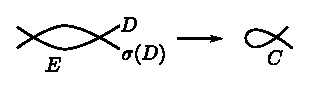
\includegraphics{figure/fig7.eps}} 

\item [ii)] $H^1(X,O_X(-C))=0$.

\item [iii)] $H^1(X,O_{\bar{X}}(-\bar{C}))\neq 0$, where as usual
  $\bar{X}$ is obtained from $X$ by successive blowing ups of points
  and $C$, the proper transform of $\bar{C}$ on $X$ is non-singular.
\end{itemize}

\begin{proof}
\begin{itemize}
\item [i)] Every point of intersection of $\sigma^i(D)$'s gives a
  singular\break point of $C$.

\item [ii)] $H^1(X,O_X(-C))$ is the kernel of the map $H^1(X,O_X)
  \longrightarrow H^1(C,\break O_C)$. But since $\alpha\in H^1(X,O_X)$
  generates $H^1(X,O_X)$ and since the image of $\alpha$ in
  $H^1(C,O_C)$ corresponds to the cover $E\longrightarrow C$, which is
  non-trivial, $H^1(X,O_X(-C))=0$. 

\item [iii)] First note that blowing up a point $P$ on $X$ is
  equivalent to the following: blow up $Y$ at all point of
  $\pi^{-1}(P)$. Then $G$ still acts on this surface and so take the
  quotient. So we could blow up $Y$ at all points of
  intersection\pageoriginale of $\sigma^i(D)$'s sufficiently many
  times to obtain a surface $Y$, so that $\bar{E}$ the proper
  transform of $E$ has become a disjoint union of non-singular
  irreducible curves on $Y$. Let $X=Y^G$. Then it is easy to see that
  $\bar{E}^G=\bar{C}$ where $\bar{C}$ is the smooth model of $C$. Now
  the cover $\bar{Y}\longrightarrow\bar{X}$ is still etale and hence
  gives a non-trivial element $\beta\in H^1(X,O_X)$. But then image of
  $\beta$ in $H^1(C,O_C)$ is trivial since the corresponding cover
  $\bar{E}\longrightarrow\bar{C}$ is trivial. Thus $\beta\in H^1
  (\bar{X}, O_{\bar{X}}(-\bar{C}))$ and hence $H^1(\bar{X},O_{\bar{X}}
  (-\bar{C}))\neq 0$. This proves our claim.
\end{itemize}
\end{proof}

\begin{REM*}
\begin{enumerate}
\item $O_{\bar{X}}(\bar{C})$ is not ample because a non-zero element
  of $H^1 (\bar{X},\bar{O}_X)$ which is stable under Frobenius and
  belongs to $H^1(X,\break\bar{O}_{\bar{X}}(-\bar{C}))$ gives a non-zero
  element in $H^1(\bar{X},O_{\bar{X}}(-p^n\bar{C}))$ for any
  $n\in\mathbb{N}$. So $H^1(\bar{X},O_{\bar{X}}(-m\bar{C}))$ is not
  zero for $m\gg 0$, which contradict Zariski-Enriques-Severi lemma.
\item In a way similar to the counter example above, one can construct
  another class of counter-examples.
\end{enumerate}
\end{REM*}

Let $Y$ be any abelian surface with $p$-rank positive. Then there
exists a subgroup $G$ of order $p$ in $Y$. Let $X=Y^G$ As before a
general ample curve $D$ on $Y$ can be shown to be smooth, irreducible
and not fixed by $G$. Let $C$ be the image of such a curve in
$X$. Then all the arguments we had before can be carried out for the
surface $X$ and the curve $C$, to give another example. 

